\documentclass[a4paper,11]{article} 
\usepackage[left=1in,right=1in,top=1.5cm,bottom=1cm]{geometry}
\usepackage{graphicx}
\usepackage{subcaption}
\usepackage{float}
\usepackage{listings}
\usepackage{color}
\usepackage{amsmath}
\usepackage{hyperref}

\graphicspath{{../data/}}
\hypersetup{colorlinks=true,linkcolor=blue,urlcolor=blue}
  
\definecolor{codegreen}{rgb}{0,0.6,0}
\definecolor{codegray}{rgb}{0.5,0.5,0.5}
\definecolor{codepurple}{rgb}{0.58,0,0.82}
\definecolor{backcolour}{rgb}{0.95,0.95,0.92}
 
\lstdefinestyle{mystyle}{
    backgroundcolor=\color{backcolour},   
    commentstyle=\color{codegreen},
    keywordstyle=\color{magenta},
    numberstyle=\tiny\color{codegray},
    stringstyle=\color{codepurple},
    basicstyle=\footnotesize,
    breakatwhitespace=false,         
    breaklines=true,                 
    captionpos=t,                    
    keepspaces=true,                 
    numbers=left,                    
    numbersep=5pt,                  
    showspaces=false,                
    showstringspaces=false,
    showtabs=false,                  
    tabsize=4
}
 
\lstset{style=mystyle}
\pagenumbering{gobble}
\allowdisplaybreaks

\begin{document}

\begin{center}
  \large{\textbf{CSE578 Computer Vision}}\\
  \Large{\textbf{Assignment 4 : GrabCut}}\\
  \vspace{1em}
  \large{Karnik Ram\\
  2018701007}
\end{center}

The procedure for implementing the GrabCut algorithm for foreground extraction, along with the code is explained in this report. The influence of the hyperparameters on the obtained results is then discussed. The generated results are provided at the end.

The code files are provided in the \texttt{code} directory along with this submission. The code is written in C++ and is written as a class (\texttt{GrabCut}) for modularity. To run the program,

\begin{lstlisting}[language=bash]
cd code
mkdir build && cd build
cmake ..
make
./run <image-path> <ouput-path>
# eg: ./run ../data/images/person2.png ../data/results/person2.png
\end{lstlisting}

\section{Procedure with Code}
Each step in the procedure is explained briefly in the following subsections, along with the corresponding code.

  \subsection{User interaction}
  
  The user is required to draw a bounding box around the object of interest, thereby labelling some background pixels. This is implemented using OpenCV's \texttt{highgui} module. Once the bounding box is set, the grabcut algorithm begins. The code is as follows:
  \begin{lstlisting}[language=C++]
void GrabCut::captureMouseClick(int event, int x, int y, int flags, void *userdata)
{
	switch(event)
	{
		case CV_EVENT_LBUTTONDOWN:
			{
				if(roi_state == NOT_SET)
				{
					roi_state = IN_PROCESS;
					roi = cv::Rect(x,y,1,1);
				}
			}
			break;

		case CV_EVENT_LBUTTONUP:
			{
				if(roi_state == IN_PROCESS)
				{
					roi = cv::Rect(cv::Point(roi.x,roi.y),cv::Point(x,y));
					roi_state = SET;
					showInputImage();
					std::cout << "Region set!\nPress 's' to start GrabCut!\n";
				}
			}
			break;

		case CV_EVENT_MOUSEMOVE:
			{
				if(roi_state == IN_PROCESS)
				{
					roi = cv::Rect(cv::Point(roi.x,roi.y),cv::Point(x,y));
					showInputImage();
				}
			}
			break;
	}
}
  \end{lstlisting}

  
  \subsection{Initializing Gaussian mixture models}
  
  First an alpha matte matrix is initialized with the background pixels hard labelled as $0$, and the unknown pixels (those within the bounding box) soft labelled as foreground or $3$. 5-component GMMs are then fitted for the background and foreground regions each using Kmeans. The following is the corresponding code:
  \begin{lstlisting}[language=C++]
void GrabCut::initializeGmm()
{
	// Assign initial opacity values based on selected background region
	alpha_matte.create(input_img.size(), CV_8UC1);	
	alpha_matte.setTo(BG);
	alpha_matte(roi).setTo(PFG);

	// Initialize fg and bg GMM from initial selection using kmeans
	fg_gmm.models.resize(num_components);
	bg_gmm.models.resize(num_components);

	std::vector<cv::Vec3f> fg_samples, bg_samples;

	for(int x = 0; x < input_img.rows; x++)
		for(int y = 0; y < input_img.cols; y++)
		{
			if(alpha_matte.at<uchar>(x, y) == FG || alpha_matte.at<uchar>(x, y) == PFG)
				fg_samples.push_back((cv::Vec3f)input_img.at<cv::Vec3b>(x, y));

			else
				bg_samples.push_back((cv::Vec3f)input_img.at<cv::Vec3b>(x, y));
		}

	std::vector<int> fg_cluster_indices, bg_cluster_indices;
	cv::kmeans(fg_samples, num_components, fg_cluster_indices, cv::TermCriteria(CV_TERMCRIT_ITER, 10, 0.0), 0, cv::KMEANS_PP_CENTERS);
	cv::kmeans(bg_samples, num_components, bg_cluster_indices, cv::TermCriteria(CV_TERMCRIT_ITER, 10, 0.0), 0, cv::KMEANS_PP_CENTERS);

	int i = 0, j = 0;
	pixel_to_component.create(input_img.size(), CV_8UC1);
	for(int x = 0; x < pixel_to_component.rows; x++)
		for(int y = 0; y < pixel_to_component.cols; y++)
		{
			if(alpha_matte.at<uchar>(x, y) == FG || alpha_matte.at<uchar>(x, y) == PFG)
				pixel_to_component.at<uchar>(x, y) = fg_cluster_indices[i++];
			else
				pixel_to_component.at<uchar>(x, y) = bg_cluster_indices[j++];
		}

	learnGmmParameters();
}
  \end{lstlisting}
  
  The model parameters - mean, covariance, component weights - are then estimated using standard MLE expressions. The inverse covariance and determinant of covariance matrix are also stored for convenience. The code is as follow:
  
  \begin{lstlisting}[language=C++]
 void GrabCut::learnGmmParameters()
{
	// Estimate mean, convariance, component weights
	int component;
	cv::Vec3b pixel;
	Eigen::Vector3f eg_pixel;

	for(int x = 0; x < pixel_to_component.rows; x++)
		for(int y = 0; y < pixel_to_component.cols; y++)
		{
			component = pixel_to_component.at<uchar>(x, y);
			pixel = input_img.at<cv::Vec3b>(x, y);
			eg_pixel << pixel[0], pixel[1], pixel[2];

			if(alpha_matte.at<uchar>(x, y) == FG || alpha_matte.at<uchar>(x, y) == PFG)
			{
				fg_gmm.models[component].mean += eg_pixel;
				fg_gmm.models[component].covariance += eg_pixel * eg_pixel.transpose();
				fg_gmm.models[component].sample_count++;
				fg_gmm.sample_count++;
			}

			else
			{
				bg_gmm.models[component].mean += eg_pixel;
				bg_gmm.models[component].covariance += eg_pixel * eg_pixel.transpose();
				bg_gmm.models[component].sample_count++;
				bg_gmm.sample_count++;
			}
		}
	
	for(int i = 0; i < num_components; i++)
	{
		if(fg_gmm.models[i].sample_count == 0)
			fg_gmm.models[i].weight = 0;

		else
		{
			fg_gmm.models[i].mean /= fg_gmm.models[i].sample_count;
			fg_gmm.models[i].covariance /= fg_gmm.models[i].sample_count;
			fg_gmm.models[i].covariance -= fg_gmm.models[i].mean * fg_gmm.models[i].mean.transpose();
			fg_gmm.models[i].inverse_covariance = fg_gmm.models[i].covariance.inverse();
			fg_gmm.models[i].detm_covariance = fg_gmm.models[i].covariance.determinant();
			fg_gmm.models[i].weight = (double)fg_gmm.models[i].sample_count / fg_gmm.sample_count;
		}

		if(bg_gmm.models[i].sample_count == 0)
			bg_gmm.models[i].weight = 0;

		else
		{
			bg_gmm.models[i].mean /= bg_gmm.models[i].sample_count;
			bg_gmm.models[i].covariance /= bg_gmm.models[i].sample_count;
			bg_gmm.models[i].covariance -= bg_gmm.models[i].mean * bg_gmm.models[i].mean.transpose();
			bg_gmm.models[i].inverse_covariance = bg_gmm.models[i].covariance.inverse();
			bg_gmm.models[i].detm_covariance = bg_gmm.models[i].covariance.determinant();
			bg_gmm.models[i].weight = (double)bg_gmm.models[i].sample_count / bg_gmm.sample_count;
		}
	}
}
  \end{lstlisting}

  \vspace{1em}
  
  \subsection{Constructing a graph and solving}
  
    The unary and binary cost terms in the Gibb's segmentation energy function segmentation are then computed.  The function is then minimized using min-cut. GrabCut co-author Vladimir's C-library implementation for max-flow/min-cut is made use of for this purpose. The unary cost terms correspond to the terminal edges, and the binary cost terms correspond to the pixel-pixel edges. The code is as follows:
    \begin{lstlisting}[language=C++]
    
void GrabCut::estimateNeighborWeights(const double &beta, const double &gamma, cv::Mat &left_weights,
		cv::Mat &up_weights, cv::Mat &up_left_weights, cv::Mat &up_right_weights)
{
	cv::Vec3b pixel, diff;

	for(int x = 0; x < input_img.rows; x++)
		for(int y = 0; y < input_img.cols; y++)
		{
			pixel = input_img.at<cv::Vec3b>(x, y);
			if(x > 0)
			{
				diff = pixel - input_img.at<cv::Vec3b>(x - 1, y);
				left_weights.at<double>(x, y) = gamma * exp(-beta*diff.dot(diff));
			}

			if(y > 0)
			{
				diff = pixel - input_img.at<cv::Vec3b>(x, y - 1);
				up_weights.at<double>(x, y) = gamma * exp(-beta*diff.dot(diff));
			}
			
			if(x>0 && y>0)
			{
				diff = pixel - input_img.at<cv::Vec3b>(x - 1, y - 1);
				up_left_weights.at<double>(x, y) = (gamma/sqrt(2)) * exp(-beta*diff.dot(diff));
			}

			if(x>0 && y<input_img.cols-1)
			{
				diff = pixel - input_img.at<cv::Vec3b>(x + 1, y - 1);
				up_right_weights.at<double>(x, y) = (gamma/sqrt(2)) * exp(-beta*diff.dot(diff));
			}
		}
}

void GrabCut::constructGraph(const double &lambda, const cv::Mat &left_weights,
		const cv::Mat &up_weights, const cv::Mat &up_left_weights,
		const cv::Mat &up_right_weights, GraphType *graph)
{
	cv::Vec3b pixel;
	Eigen::Vector3f eg_pixel;
	int node_id;
	Gaussian model;
	double source_weight, sink_weight, n_weight;

	for(int x = 0; x < input_img.rows; x++)
		for(int y = 0; y < input_img.cols; y++)
		{
			pixel = input_img.at<cv::Vec3b>(x,y);
			eg_pixel << pixel[0], pixel[1], pixel[2];
			node_id = graph->add_node();
			source_weight = sink_weight = n_weight = 0;

			if(alpha_matte.at<uchar>(x, y) == FG)
			{
				source_weight = lambda;
				sink_weight = 0;
			}

			else if(alpha_matte.at<uchar>(x, y) == BG)
			{
				source_weight = 0;
				sink_weight = lambda;
			}

			else if(alpha_matte.at<uchar>(x, y) == PFG || alpha_matte.at<uchar>(x,y) == PBG)
			{
				for(int i = 0; i < num_components; i++)
				{
					model = fg_gmm.models[i];
					if(model.weight > 0)
					{
						sink_weight += model.weight * 1.0f/sqrt(model.detm_covariance)
							* exp(-0.5f*(eg_pixel - model.mean).transpose() * model.inverse_covariance * (eg_pixel - model.mean));
					}
					
					model = bg_gmm.models[i];
					if(model.weight > 0)
					{
						source_weight += model.weight * 1.0f/sqrt(model.detm_covariance)
							* exp(-0.5f*(eg_pixel - model.mean).transpose() * model.inverse_covariance * (eg_pixel - model.mean));
					}
				}

				source_weight = -log(source_weight);
				sink_weight = -log(sink_weight);
			}

			graph->add_tweights(node_id, source_weight, sink_weight);

			if(x > 0)
			{
				n_weight = left_weights.at<double>(x, y);
				graph->add_edge(node_id, node_id - input_img.cols, n_weight, n_weight);
			}

			if(y > 0)
			{
				n_weight = up_weights.at<double>(x, y);
				graph->add_edge(node_id, node_id - 1, n_weight, n_weight);
			}
			
			if(x>0 && y>0)
			{
				n_weight = up_left_weights.at<double>(x, y);
				graph->add_edge(node_id, node_id - input_img.cols - 1, n_weight, n_weight);
			}

			if(x>0 && y<input_img.cols-1)
			{
				n_weight = up_right_weights.at<double>(x, y);
				graph->add_edge(node_id, node_id -input_img.cols + 1, n_weight, n_weight);
			}
		}
}

void GrabCut::estimateSegmentation(GraphType *graph)
{
	int flow = graph->maxflow();

	for(int x = 0; x < alpha_matte.rows; x++)
		for(int y = 0; y < alpha_matte.cols; y++)
		{
			if(alpha_matte.at<uchar>(x, y) == PBG || alpha_matte.at<uchar>(x, y) == PFG)
			{
				if(graph->what_segment(x*alpha_matte.cols + y) == GraphType::SOURCE)
					alpha_matte.at<uchar>(x, y) = PFG;

				else
					alpha_matte.at<uchar>(x, y) = PBG;
			}
		}

	//extract foreground image
	foreground = cv::Mat::zeros(input_img.size(), CV_8UC3);

	for(int i = 0; i < input_img.rows; i++)
		for(int j = 0; j < input_img.cols; j++)
			if(alpha_matte.at<uchar>(i, j) == PFG || alpha_matte.at<uchar>(i, j) == FG)
				foreground.at<cv::Vec3b>(i, j) = input_img.at<cv::Vec3b>(i, j);
}
    \end{lstlisting}
    \vspace{1em}
  
  \subsection{Re-estimation and learning}
  
 Using the estimated segmentation, the alpha matte values are re-assigned according to the estimated foregound and background regions and then the GMMs are remodelled. The most likely component is assigned to each fg/bg pixel and the model parameters are re-estimated. The code is as follows:
    \begin{lstlisting}[language=C++]
void GrabCut::assignGmmComponents()
{
	cv::Vec3b pixel;
	Eigen::Vector3f eg_pixel;
	Gaussian model;

	double p, p_max, best_component;

	for(int x = 0; x < input_img.rows; x++)
		for(int y = 0; y < input_img.cols; y++)
		{
			pixel = input_img.at<cv::Vec3b>(x, y);
			eg_pixel << pixel[0], pixel[1], pixel[2];

			if(alpha_matte.at<uchar>(x, y) == FG || alpha_matte.at<uchar>(x, y) == PFG)
			{
				p_max = 0;

				for(int i = 0; i < num_components; i++)
				{
					model = fg_gmm.models[i];
					if(model.weight > 0)
					{
						p = 1.0f/sqrt(model.detm_covariance)
							* exp(-0.5f*(eg_pixel - model.mean).transpose() * model.inverse_covariance
									* (eg_pixel - model.mean));
					}

					if(p > p_max)
					{
						p_max = p;
						best_component = i;
					}
				}

				pixel_to_component.at<uchar>(x, y) = best_component;
			}

			else
			{
				p_max = 0;

				for(int i = 0; i < num_components; i++)
				{
					model = bg_gmm.models[i];
					if(model.weight > 0)
					{
						p = 1.0f/sqrt(model.detm_covariance)
							* exp(-0.5f*(eg_pixel - model.mean).transpose() * model.inverse_covariance
									* (eg_pixel - model.mean));
					}

					if(p > p_max)
					{
						p_max = p;
						best_component = i;
					}
				}

				pixel_to_component.at<uchar>(x, y) = best_component;
			}
		}
}

    \end{lstlisting}
    \vspace{1em}
    
  \subsection{Iterative process}
  
  This process is repeated iteratively within a loop, with the user choosing whether to continue for another iteration or to stop, after each iteration. The code is as follows:
  
    \begin{lstlisting}[language=C++]
void GrabCut::runGrabCut()
{
	int num_nodes = input_img.cols * input_img.rows;
	int num_edges = 4*input_img.cols*input_img.rows - 3*input_img.cols -3*input_img.rows + 2;
	//int num_edges = 2*input_img.cols*input_img.rows - input_img.cols - input_img.rows;
	double beta = estimateBeta();
	double gamma = 20;
	double lambda = 200;

	cv::Mat left_weights = cv::Mat::zeros(input_img.size(), CV_64FC1);
	cv::Mat up_weights = cv::Mat::zeros(input_img.size(), CV_64FC1);
	cv::Mat up_left_weights = cv::Mat::zeros(input_img.size(), CV_64FC1);
	cv::Mat up_right_weights = cv::Mat::zeros(input_img.size(), CV_64FC1);

	int iter = 1;
	std::cout << "Running iteration #" << iter++ << std::endl;

	estimateNeighborWeights(beta, gamma, left_weights, up_weights, up_left_weights, up_right_weights);

	initializeGmm();
	std::cout << "Initialization complete!\n";

	cv::namedWindow("Foreground", CV_WINDOW_NORMAL);

	while(1)	
	{

		GraphType *graph = new GraphType(num_nodes, num_edges);
		constructGraph(lambda, left_weights, up_weights, up_left_weights, up_right_weights, graph);
		estimateSegmentation(graph);
		std::cout << "Segmentation complete!\n";

		cv::imshow("Foreground", foreground);
		std::cout << "\nPress 'c' for another iteration\nPress 'Esc' to save output and exit\n\n";

		while(1)
		{
			char c = cv::waitKey(0);

			if(c == 'c')
			{
				std::cout << "Running iteration #" << iter++ << std::endl;
				break;
			}

			else if(c == '\x1b')
			{
				std::cout << "Saving output..\n";
				cv::imwrite(output_path, foreground);
				boost::filesystem::path p(output_path);
				std::string file_name = p.filename().string();
				cv::Mat temp_img;
				input_img.copyTo(temp_img);
				cv::rectangle(temp_img,cv::Point(roi.x,roi.y),cv::Point(roi.x + roi.width,
					roi.y + roi.height),cv::Scalar(0,0,255),2);
				cv::imwrite("../data/results/input/" + file_name, temp_img);

				return;
			}
		}

		assignGmmComponents();
		learnGmmParameters();
	}
}
    \end{lstlisting}
    \vspace{2em}
    
     
\section{Hyperparameters}
\subsection{Number of iterations}
Images in which the foregound object is only a small fraction of the bounding box region required more number of iterations. Images with a large foreground, like the \texttt{flower} example gave a good result in one step. However, the segmentation doesn't converge to a fixed segmentation - more likely to be a bug in my implementation.

\subsection{Number of components}
Performance decreased with more number of components, especially for images with fewer colors. In a sense, more components causes multiple components to be assigned to the same object which leads to harder segmentation. Number of components was set to 5 for generating results.

\subsection{Number of neighbors}
8-neighborhood gave better results than 4-neighborhood and also required fewer iterations. 8-neighborhood was used for generating results.

\subsection{Color space}
Though in theory, color spaces like HSV and LAB can lead to better segmentation results, I did not get any better results in my experiments. YCrCb space gave worse results.
  
\section{Results}
All the input and result images show here can also be found here - \href{https://drive.google.com/drive/folders/1ctn--zOvO0Ccc5qZbPCyCRNH6bSbNcWa?usp=sharing}{link}.
  
  \begin{center}
  \begin{figure}[H]
    \begin{subfigure}{.33\textwidth}
      \centering
      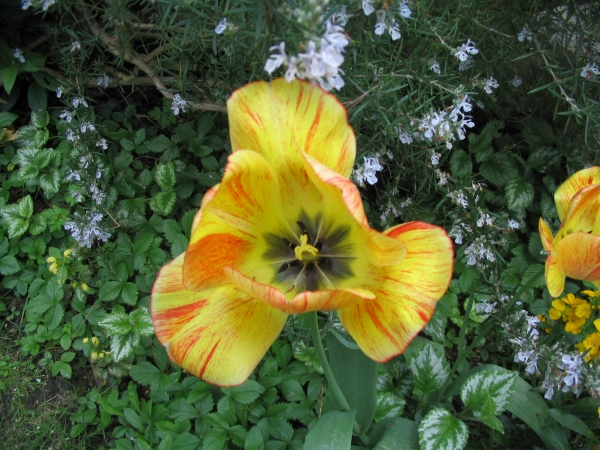
\includegraphics[width=0.9\linewidth]{images/flower.jpg}
    \end{subfigure}
    \begin{subfigure}{.33\textwidth}
      \centering
      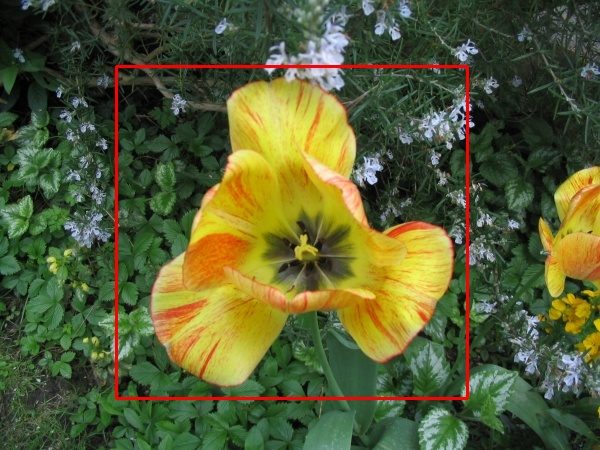
\includegraphics[width=0.9\linewidth]{results/input/flower}
    \end{subfigure}
    \begin{subfigure}{0.33\textwidth}
      \centering
      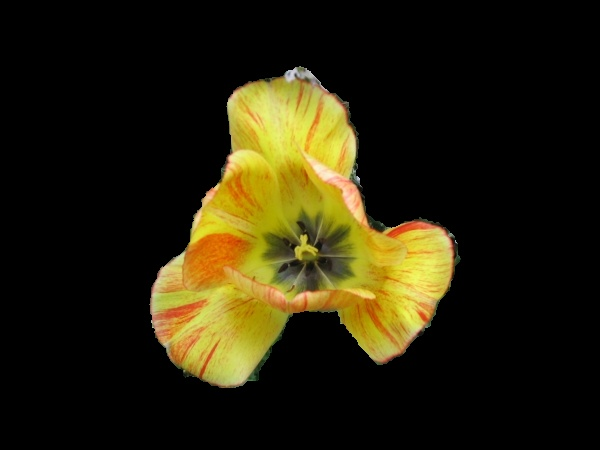
\includegraphics[width=0.9\linewidth]{results/flower}
    \end{subfigure}\\
      \vspace{1em}
      
    \begin{subfigure}{0.33\textwidth}
      \centering
      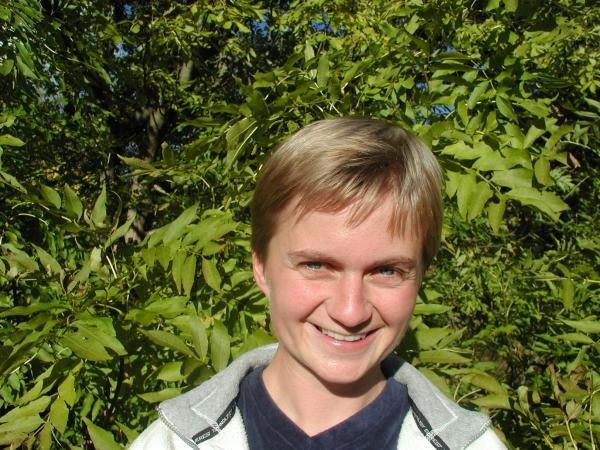
\includegraphics[width=0.9\linewidth]{images/person2}
    \end{subfigure}
    \begin{subfigure}{.33\textwidth}
      \centering
      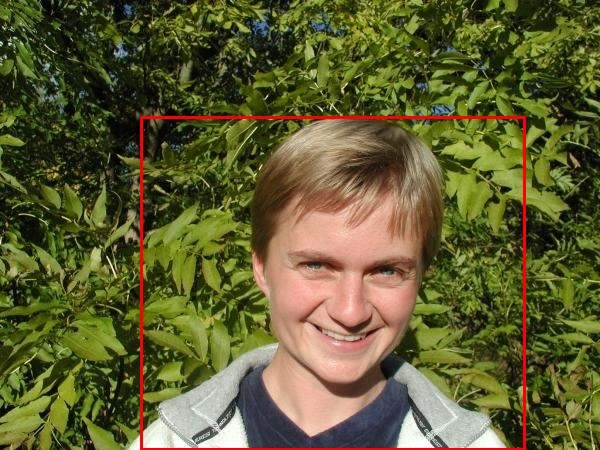
\includegraphics[width=0.9\linewidth]{results/input/person2}
    \end{subfigure}
    \begin{subfigure}{0.33\textwidth}
      \centering
      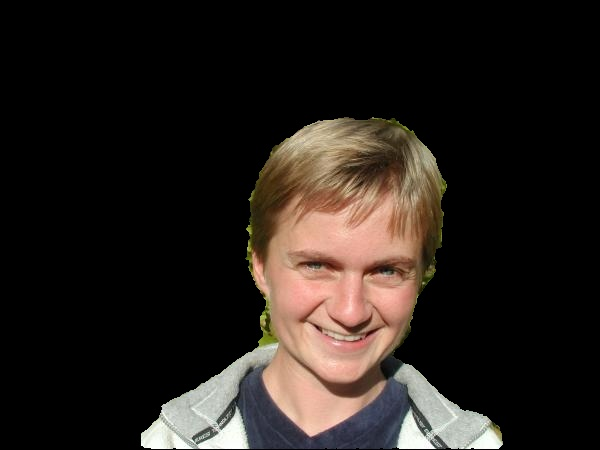
\includegraphics[width=0.9\linewidth]{results/person2}
    \end{subfigure}\\
    \vspace{1em}
    
   \begin{subfigure}{0.33\textwidth}
      \centering
      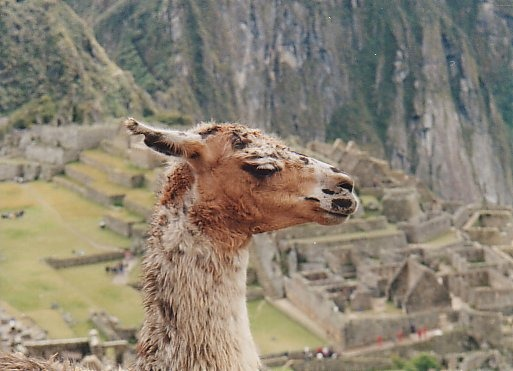
\includegraphics[width=0.9\linewidth]{images/llama}
    \end{subfigure}
    \begin{subfigure}{.33\textwidth}
      \centering
      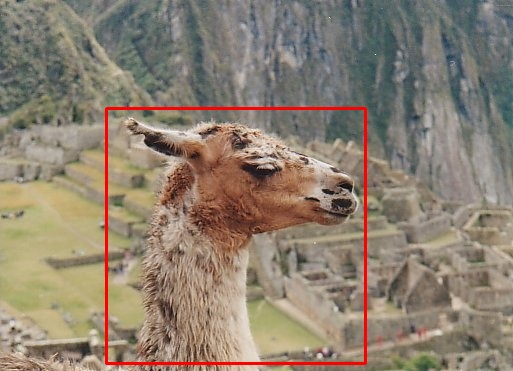
\includegraphics[width=0.9\linewidth]{results/input/llama}
    \end{subfigure}
    \begin{subfigure}{0.33\textwidth}
      \centering
      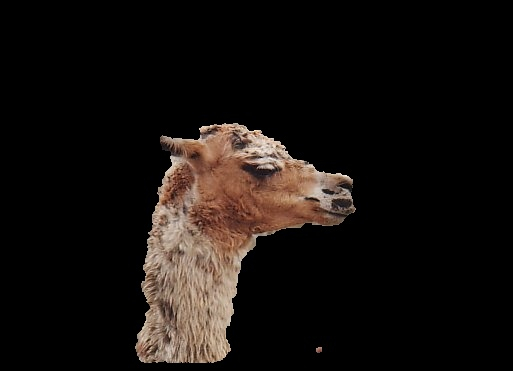
\includegraphics[width=0.9\linewidth]{results/llama}
   \end{subfigure}\\
    \vspace{1em}
    
   \begin{subfigure}{0.33\textwidth}
      \centering
      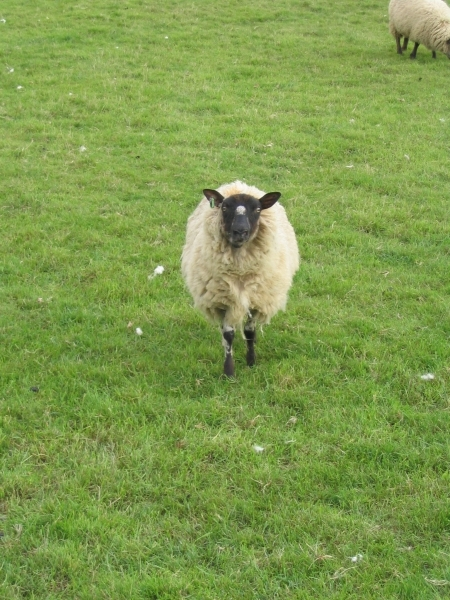
\includegraphics[width=0.9\linewidth]{images/sheep}
    \end{subfigure}
    \begin{subfigure}{.33\textwidth}
      \centering
      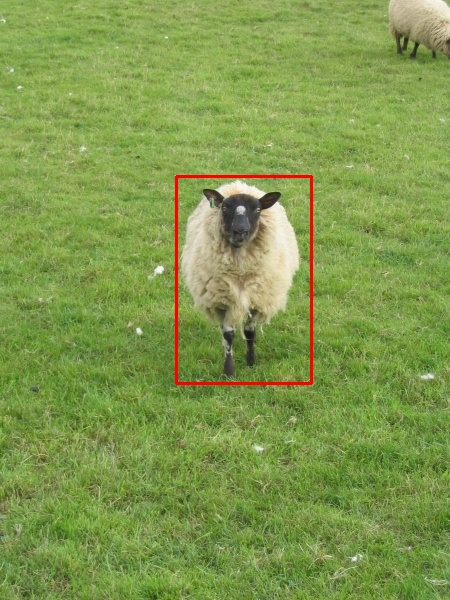
\includegraphics[width=0.9\linewidth]{results/input/sheep}
    \end{subfigure}
    \begin{subfigure}{0.33\textwidth}
      \centering
      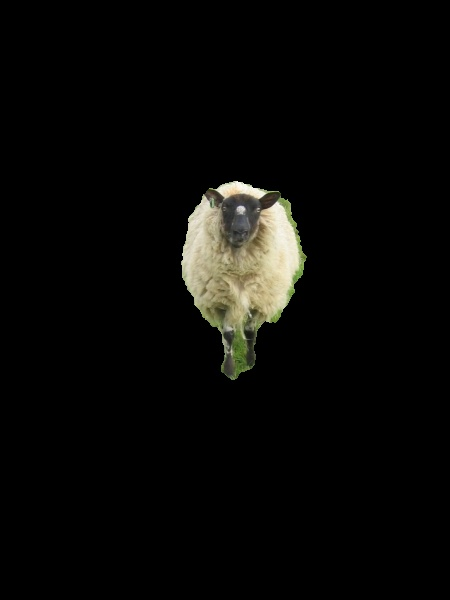
\includegraphics[width=0.9\linewidth]{results/sheep}
   \end{subfigure}\\
    \vspace{1em}
    
   \begin{subfigure}{0.33\textwidth}
      \centering
      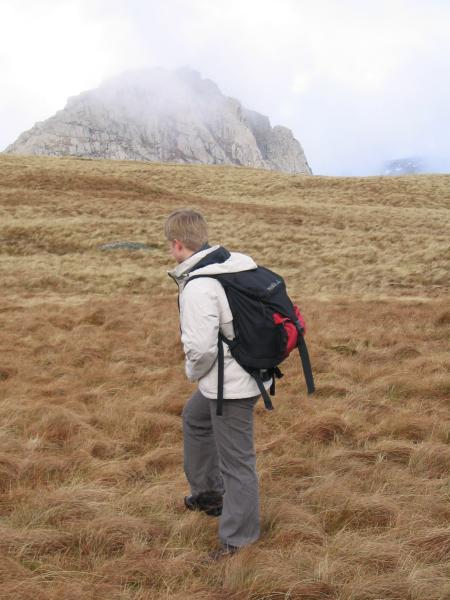
\includegraphics[width=0.9\linewidth]{images/person3}
    \end{subfigure}
    \begin{subfigure}{.33\textwidth}
      \centering
      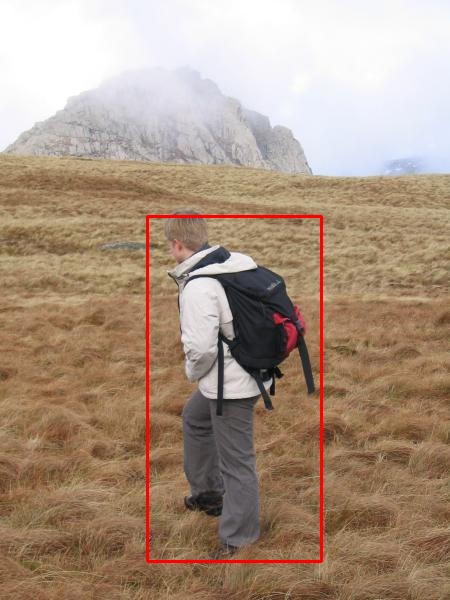
\includegraphics[width=0.9\linewidth]{results/input/person3}
    \end{subfigure}
    \begin{subfigure}{0.33\textwidth}
      \centering
      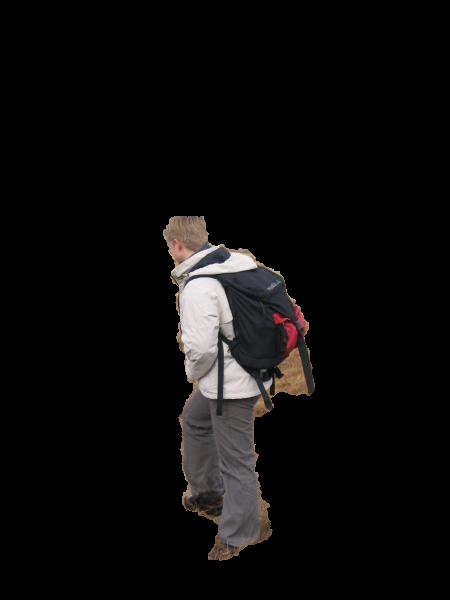
\includegraphics[width=0.9\linewidth]{results/person3}
   \end{subfigure}
    \caption{Results}
  \end{figure}
  \end{center}
  \begin{center}
  \begin{figure}[H]
    \begin{subfigure}{.33\textwidth}
      \centering
      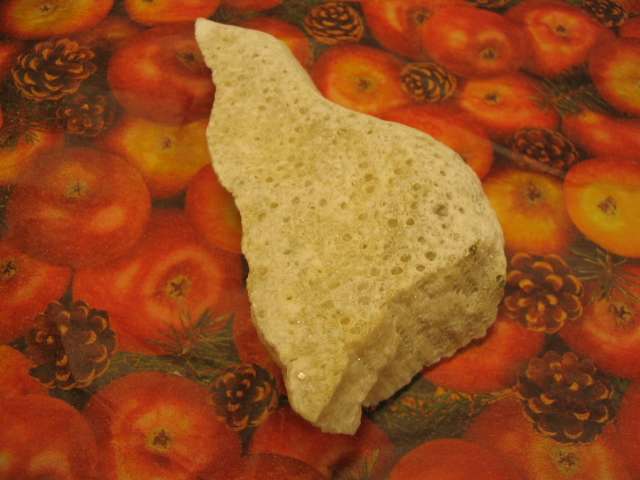
\includegraphics[width=0.9\linewidth]{images/stone2.jpg}
    \end{subfigure}
    \begin{subfigure}{.33\textwidth}
      \centering
      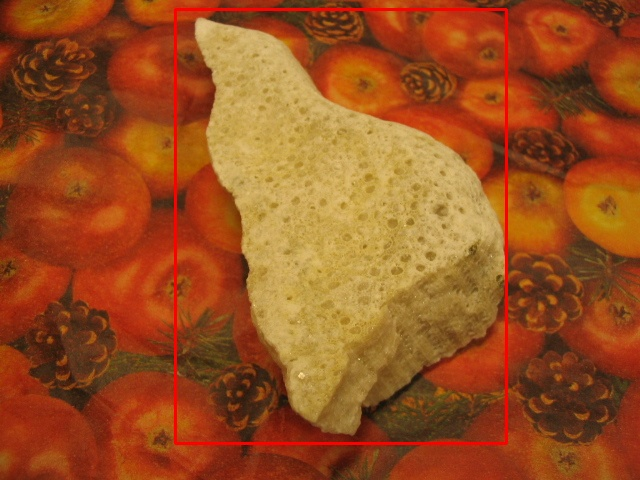
\includegraphics[width=0.9\linewidth]{results/input/stone2}
    \end{subfigure}
    \begin{subfigure}{0.33\textwidth}
      \centering
      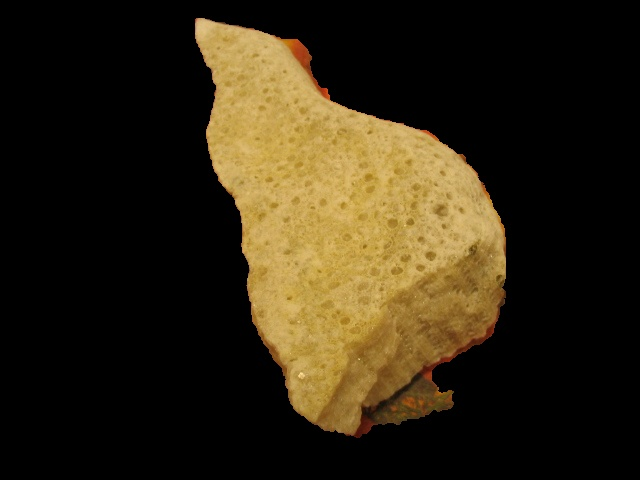
\includegraphics[width=0.9\linewidth]{results/stone2}
    \end{subfigure}\\
      \vspace{1em}
      
    \begin{subfigure}{0.33\textwidth}
      \centering
      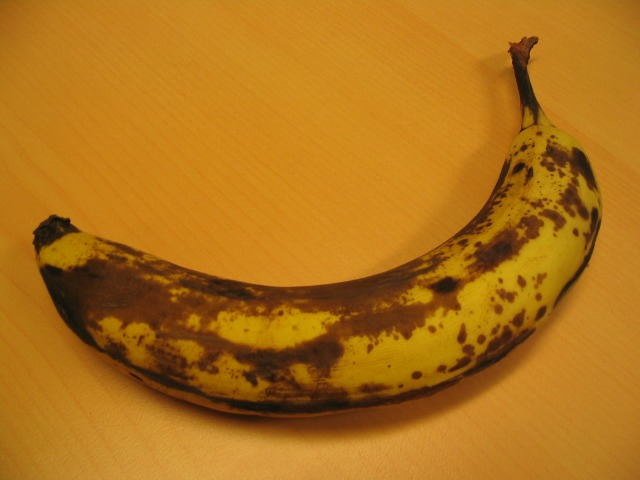
\includegraphics[width=0.9\linewidth]{images/banana1}
    \end{subfigure}
    \begin{subfigure}{.33\textwidth}
      \centering
      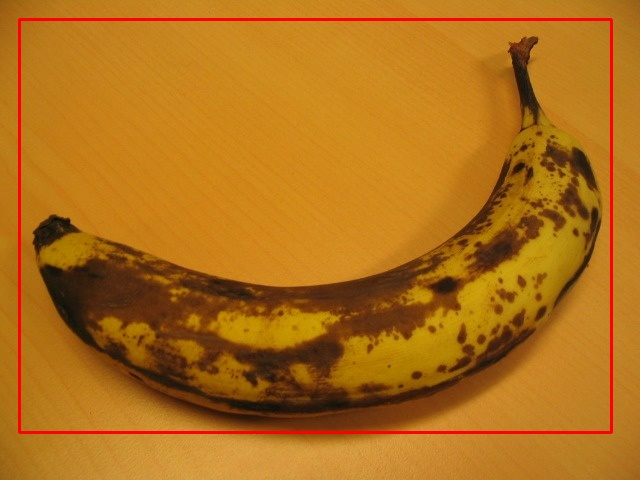
\includegraphics[width=0.9\linewidth]{results/input/banana1}
    \end{subfigure}
    \begin{subfigure}{0.33\textwidth}
      \centering
      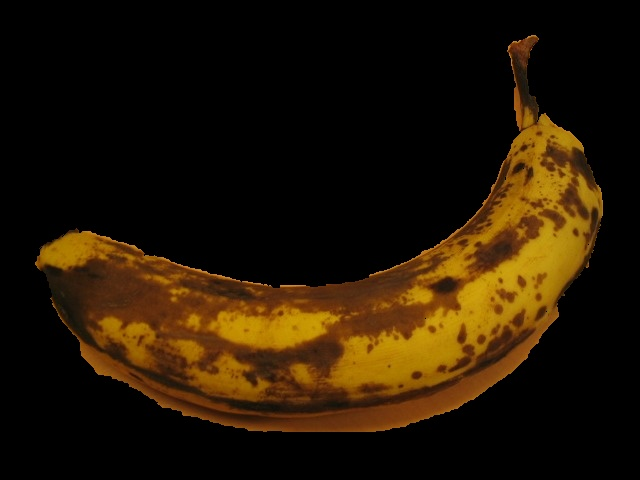
\includegraphics[width=0.9\linewidth]{results/banana1}
    \end{subfigure}\\
    \vspace{1em}
    
   \begin{subfigure}{0.33\textwidth}
      \centering
      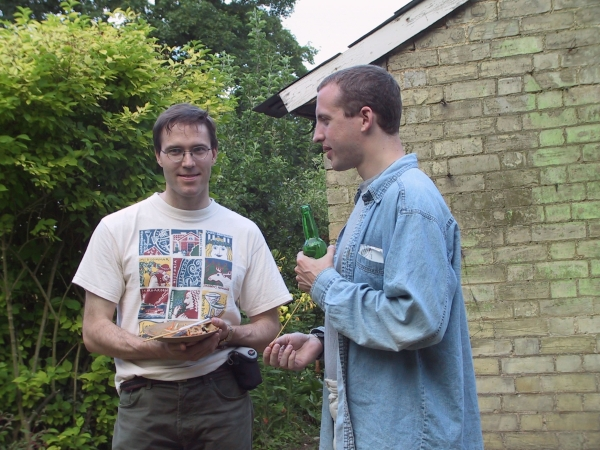
\includegraphics[width=0.9\linewidth]{images/person4}
    \end{subfigure}
    \begin{subfigure}{.33\textwidth}
      \centering
      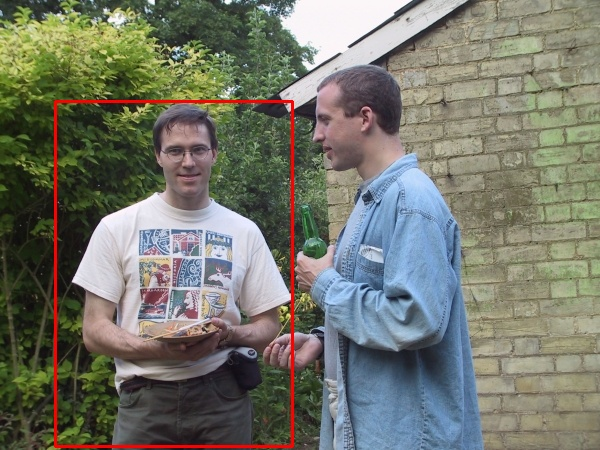
\includegraphics[width=0.9\linewidth]{results/input/person4}
    \end{subfigure}
    \begin{subfigure}{0.33\textwidth}
      \centering
      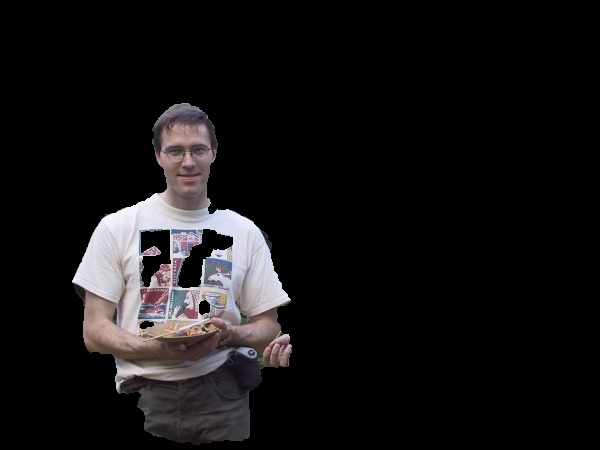
\includegraphics[width=0.9\linewidth]{results/person4}
   \end{subfigure}\\
    \vspace{1em}
    
   \begin{subfigure}{0.33\textwidth}
      \centering
      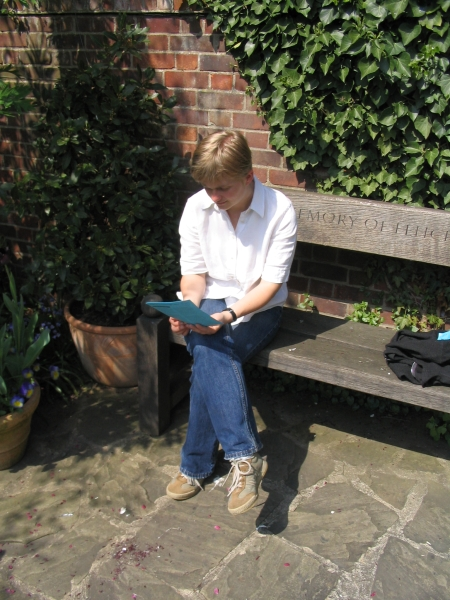
\includegraphics[width=0.9\linewidth]{images/person6}
    \end{subfigure}
    \begin{subfigure}{.33\textwidth}
      \centering
      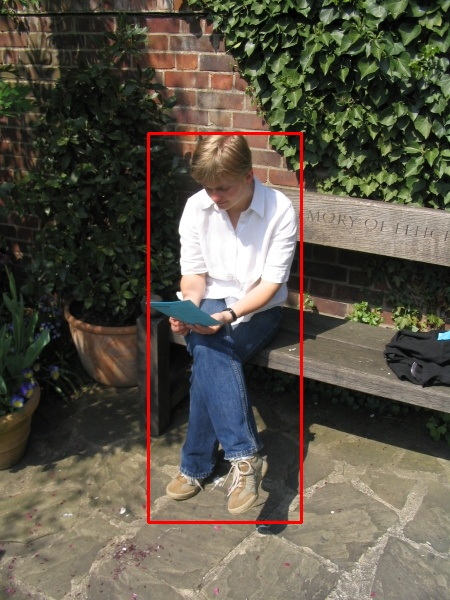
\includegraphics[width=0.9\linewidth]{results/input/person6}
    \end{subfigure}
    \begin{subfigure}{0.33\textwidth}
      \centering
      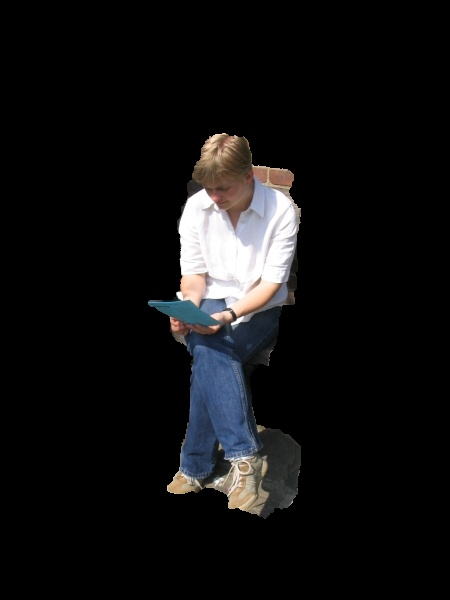
\includegraphics[width=0.9\linewidth]{results/person6}
   \end{subfigure}\\
    \vspace{1em}
    
   \begin{subfigure}{0.33\textwidth}
      \centering
      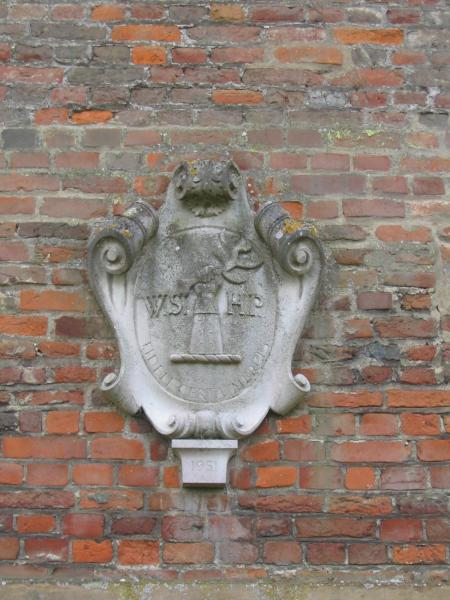
\includegraphics[width=0.9\linewidth]{images/memorial}
    \end{subfigure}
    \begin{subfigure}{.33\textwidth}
      \centering
      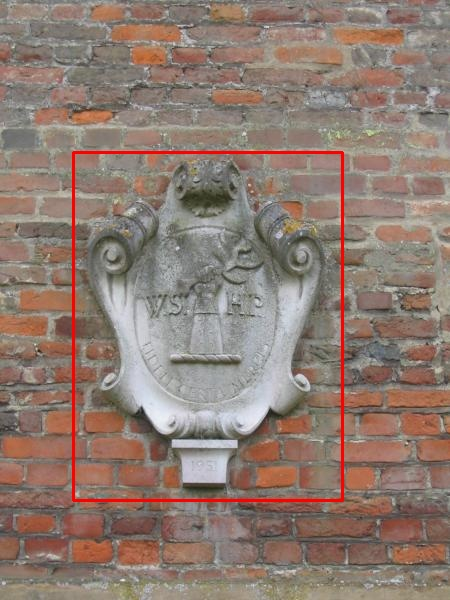
\includegraphics[width=0.9\linewidth]{results/input/memorial}
    \end{subfigure}
    \begin{subfigure}{0.33\textwidth}
      \centering
      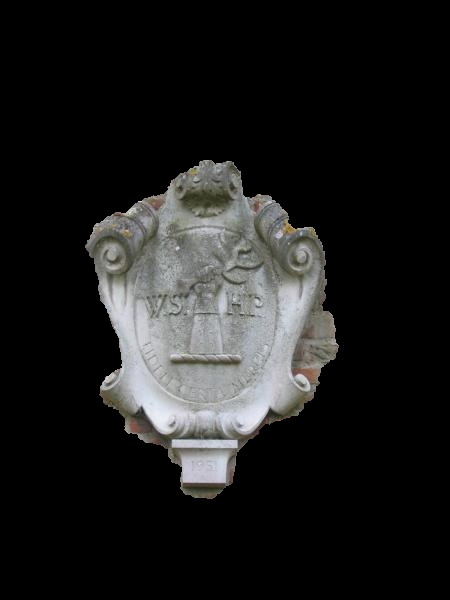
\includegraphics[width=0.9\linewidth]{results/memorial}
   \end{subfigure}
    \caption{Some more results}
  \end{figure}
  \end{center}
  
  \begin{center}
  \begin{figure}[H]
    \begin{subfigure}{.33\textwidth}
      \centering
      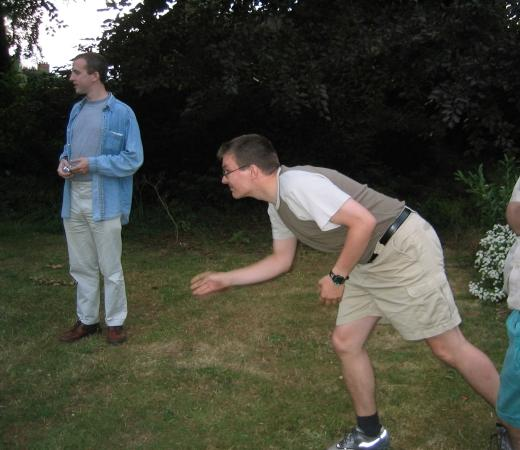
\includegraphics[width=0.9\linewidth]{images/bool}
    \end{subfigure}
    \begin{subfigure}{.33\textwidth}
      \centering
      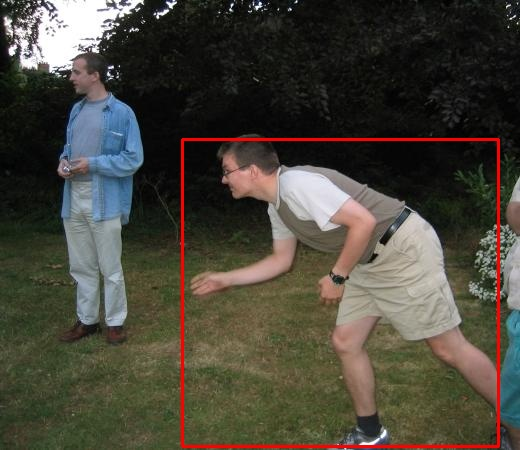
\includegraphics[width=0.9\linewidth]{results/input/bool}
    \end{subfigure}
    \begin{subfigure}{0.33\textwidth}
      \centering
      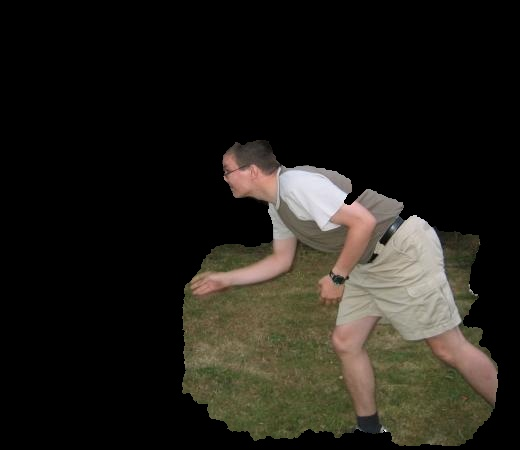
\includegraphics[width=0.9\linewidth]{results/bool}
    \end{subfigure}\\
      \vspace{1em}
      
    \begin{subfigure}{0.33\textwidth}
      \centering
      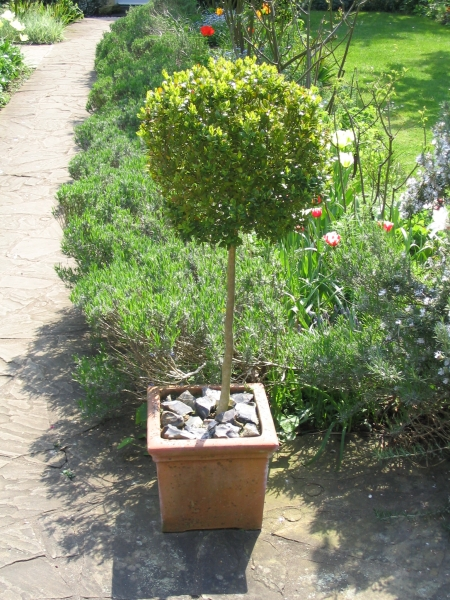
\includegraphics[width=0.9\linewidth]{images/bush}
    \end{subfigure}
    \begin{subfigure}{.33\textwidth}
      \centering
      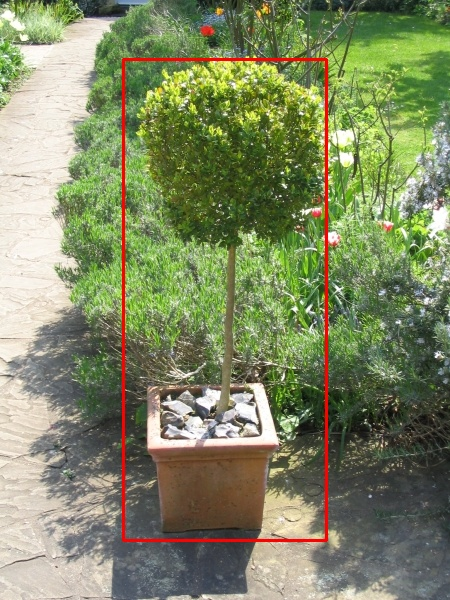
\includegraphics[width=0.9\linewidth]{results/input/bush}
    \end{subfigure}
    \begin{subfigure}{0.33\textwidth}
      \centering
      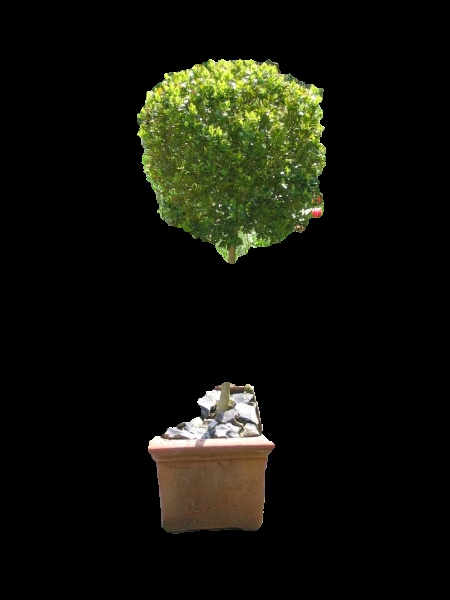
\includegraphics[width=0.9\linewidth]{results/bush}
    \end{subfigure}\\
    \vspace{1em}
    
   \begin{subfigure}{0.33\textwidth}
      \centering
      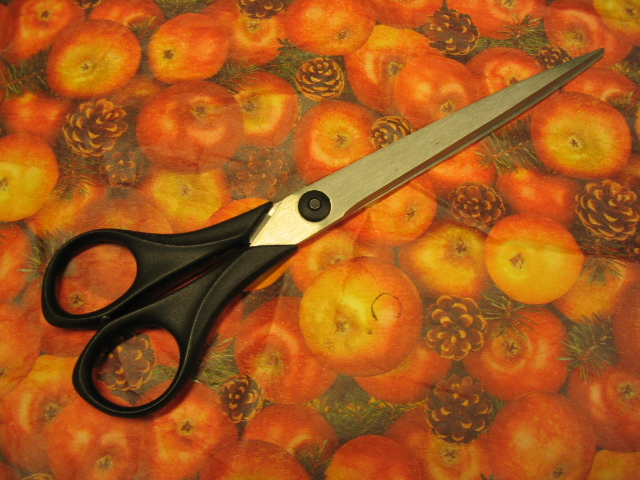
\includegraphics[width=0.9\linewidth]{images/scissors}
    \end{subfigure}
    \begin{subfigure}{.33\textwidth}
      \centering
      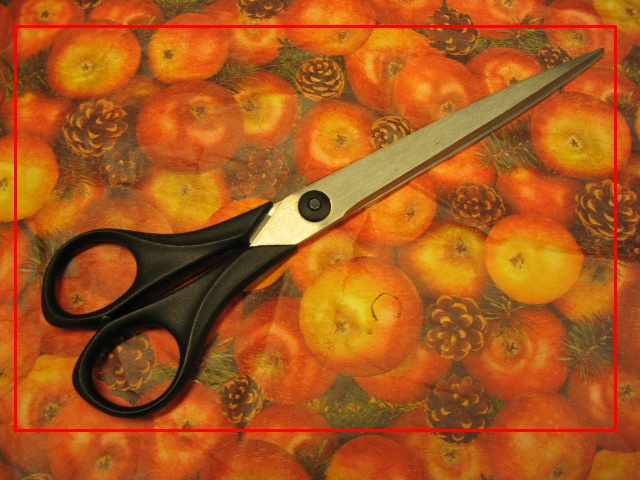
\includegraphics[width=0.9\linewidth]{results/input/scissors}
    \end{subfigure}
    \begin{subfigure}{0.33\textwidth}
      \centering
      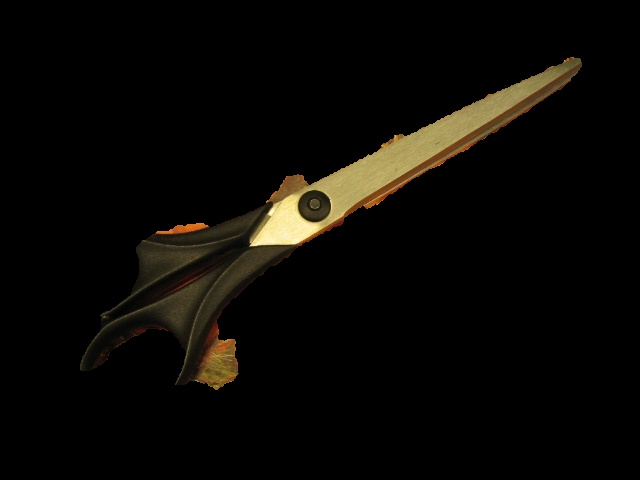
\includegraphics[width=0.9\linewidth]{results/scissors}
   \end{subfigure}\\
    \vspace{1em}
    
   \begin{subfigure}{0.33\textwidth}
      \centering
      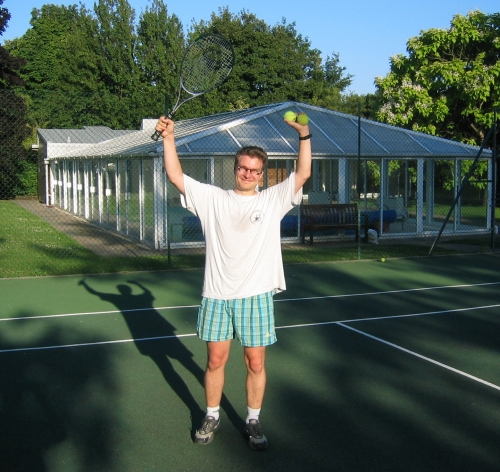
\includegraphics[width=0.9\linewidth]{images/tennis}
    \end{subfigure}
    \begin{subfigure}{.33\textwidth}
      \centering
      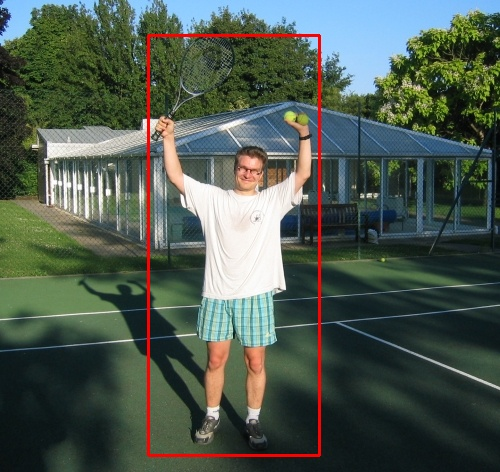
\includegraphics[width=0.9\linewidth]{results/input/tennis}
    \end{subfigure}
    \begin{subfigure}{0.33\textwidth}
      \centering
      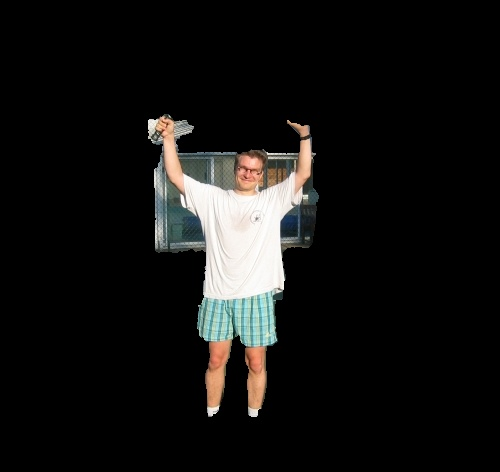
\includegraphics[width=0.9\linewidth]{results/tennis}
   \end{subfigure}\\
    \vspace{1em}
    
   \begin{subfigure}{0.33\textwidth}
      \centering
      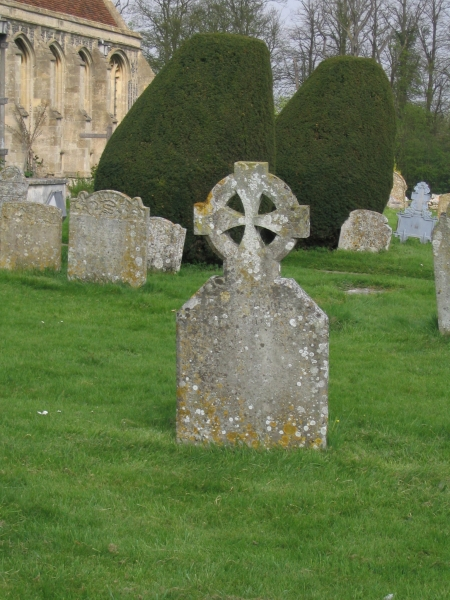
\includegraphics[width=0.9\linewidth]{images/grave}
    \end{subfigure}
    \begin{subfigure}{.33\textwidth}
      \centering
      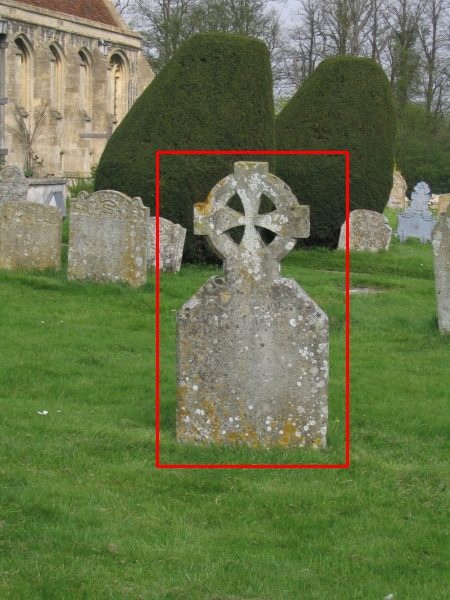
\includegraphics[width=0.9\linewidth]{results/input/grave}
    \end{subfigure}
    \begin{subfigure}{0.33\textwidth}
      \centering
      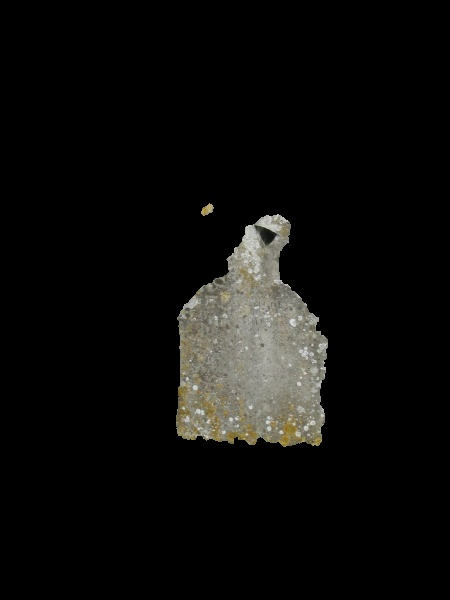
\includegraphics[width=0.9\linewidth]{results/grave}
   \end{subfigure}
    \caption{Some bad results}
  \end{figure}
  \end{center}
\end{document}